\section{MathScript\textendash a command line utility}  

MathScript has much of the functionality of other command line scripting
languages such as Matlab and MatrixX.  Standard commands useful to control
design include:
\begin{enumerate}
\item \emph{tf} creates a transfer function;
\item \emph{step} plots the step  response of a transfer function or state space
  system;
\item \emph{bode} plots the bode plot of a transfer function;
\item \emph{rlocus} plots the root locus of a transfer function;
\item \emph{nyquist} plots the nyquist plot of a transfer function.
\end{enumerate}

Example code that might be illuminating includes:

Here are some different ways of doing Example 2.1 in the FPE textbook.
You can get a step response entirely numerically, like the book does:
\begin{verbatim}
num=1/1000;
den=[1 50/1000];
sys=tf(num*500,den);
step(sys)
\end{verbatim}

You can use variables:
\begin{verbatim}
m=1000;
b=50;
num=1/m;
den=[1 b/m];
sys=tf(num*500,den)
\end{verbatim}

You can define the transfer function as a fraction (i.e., the way you would
write it down). This is ultimately going to be preferrable.
\begin{verbatim}
s=tf('s');
g=(500/m)/(s+b/m)
step(g)
\end{verbatim}

Lastly, you can incorporate ``.m'' file code into your LabVIEW VI by using the
MathScript block from the Structures palette.  An example of this is given in
Fig.~\ref{fig-mathscriptinsimTF}.  In order to do this, one must create the
MathScript block, write the desired code, create an output of the block (by
right clicking on the edge of the block), and finally define that output to be
of the appropriate data type (in the case of Fig.~\ref{fig-mathscriptinsimTF}
a ``TF Object'', and in the case of
Figs.~\ref{fig-mathscriptinsimSS}, \ref{fig-mathscriptinsimSS2TF}, and
\ref{fig-mathscriptinsimSS2TFdeg} a ``SS Object'').



\begin{figure}[h!]
\centering
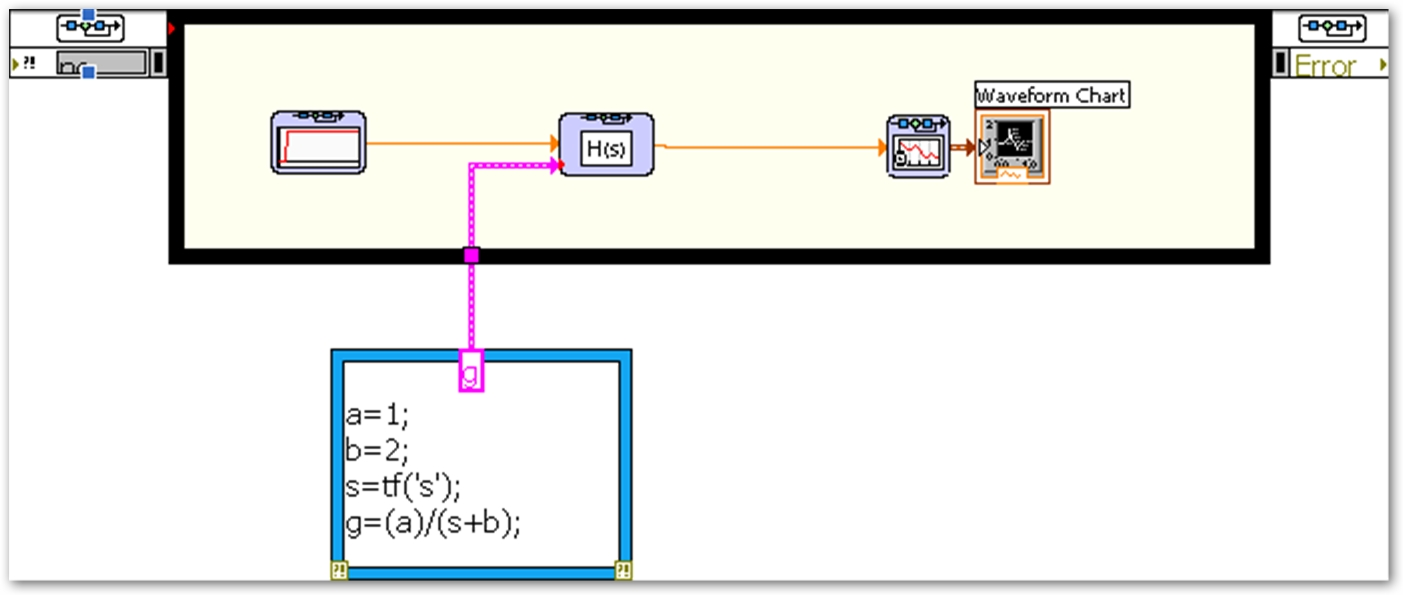
\includegraphics[width=6in]{mathscriptinsim/mathscriptinsimTF}
\caption{MathScript defining a transfer function in the simulation module}
\label{fig-mathscriptinsimTF}
\end{figure}

\begin{figure}[h!]
\centering
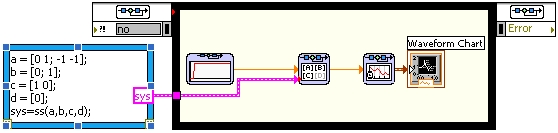
\includegraphics[width=6in]{mathscriptinsim/mathscriptinsimSS}
\caption{MathScript defining a state space system in the simulation module}
\label{fig-mathscriptinsimSS}
\end{figure}

\begin{figure}[h!]
\centering
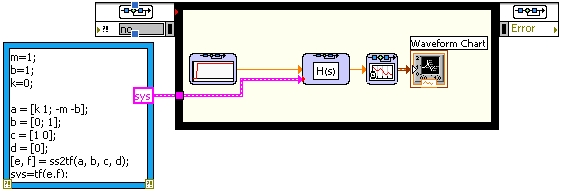
\includegraphics[width=6in]{mathscriptinsim/mathscriptinsimSS2TF}
\caption{MathScript defining a state space system, converting it to a transfer
  function, and using it in the simulation module}
\label{fig-mathscriptinsimSS2TF}
\end{figure}

\begin{figure}[h!]
\centering
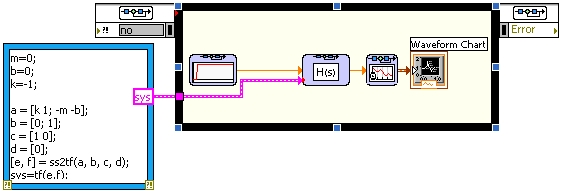
\includegraphics[width=6in]{mathscriptinsim/mathscriptinsimSS2TFdegenerate}
\caption{MathScript defining a degenerate state space system, converting it to a transfer
  function, and using it in the simulation module}
\label{fig-mathscriptinsimSS2TFdeg}
\end{figure}


 

%% Local Variables:
%% TeX-master: "../LVmanual.tex"
%% End:

